\chapter{Evaluación}
\label{cap:evaluacion}



\begin{resumen}
En este capítulo se explicará el proceso de evaluación de la aplicación: La preparación (Sección \ref{eva:prep}), el diseño de la evaluación (Sección \ref{eva:dis}), resultados obtenidos (Sección \ref{eva:res}) y el análisis de dichos resultados (Sección \ref{eva:analisis}).  
	
\end{resumen}

Al tener un prototipo funcional con la suficiente antelación a la entrega, se puso en marcha el plan de realizar una evaluación con usuarios. Durante Abril se focalizó el trabajo en mejorar la usabilidad e interfaz de la aplicación, diseñar la evaluación y en dar a conocer la aplicación al público objetivo de la aplicación. Éstos son usuarios creadores de material pictográfico, generalmente profesores de educación especial y padres y tutores. 


\section{Preparación de la evaluación}
\label{eva:prep}


Inicialmente se buscaron sitios donde se subiera material pictográfico con frecuencia para así localizar a los creadores de dicho material y contactar con ellos. La propia web de ARASAAC cuenta con una sección dedicada a la subida de material pictográfico donde se añaden nuevos materiales diariamente. La inmensa mayoría de este material contaba con una marca de agua indicando el perfil de Instagram del creador. Por ello nos decantamos por crear una cuenta de Instagram\footnote{\url{https://www.instagram.com/pictupweb/}} para crear una red de potenciales usuarios. 

En dicha cuenta, se contactó con muchos de estos creadores de material para informarles sobre el desarrollo de la aplicación. También se creó material en forma de vídeos donde se explicaban muchas funcionalidades de la web. Los vídeos contaron con una recepción positiva y de interés por parte de los usuarios, por lo que en el transcurso de un mes se logró un grupo considerable de usuarios.
\section{Diseño de la evaluación}
\label{eva:dis}

Es en este punto donde la situación causada por la situación de pandemia tuvo mayor impacto sobre el proyecto. En otras circunstancias la evaluación hubiera sido en un centro escolar de manera más cercana al usuario final, pero se tuvo que plantear una evaluación a distancia y asíncrona. El objetivo de esta evaluación es medir la usabilidad y utilidad de la aplicación. 


Debido a estas circunstancias, la evaluación se realizó mediante un formulario para que el usuario pudiera completarlo por su cuenta. Un posible problema de este tipo de evaluación estaba en la posibilidad que el usuario dejara el formulario incompleto en caso de no lograr completar alguna tarea. Otro problema era el dispositivo de evaluación, ya que la aplicación está diseñada y probada para ordenadores. Por ello, antes y durante la realización del formulario, se aconsejó encarecidamente el uso del ordenador para el desarrollo de la evaluación.

El formulario utilizado está dividido en varias partes.

Primero se plantean algunas preguntas para conocer la relación de los usuarios respecto al uso de pictogramas, la edad y ocupación. De esta manera se puede determinar el tipo de perfil de usuario que está evaluando.

Tras conocer el perfil, se plantean una serie de tareas a realizar dentro de la aplicación. Antes de plantear las tareas, se vuelve a recomendar al usuario el uso de ordenador para probar la web. 

El  posible escenario en el cual el usuario no supiera continuar con la tarea y dejara el formulario incompleto, fue solucionado mediante pistas. Las pistas son imágenes autoexplicativas donde se especifican las acciones que se han de realizar para completar cada tarea. En la Figura \ref{fig:evaPista} se puede ver la pista que indica cómo buscar un pictograma.

\begin{figure}[h!]
	\centering
	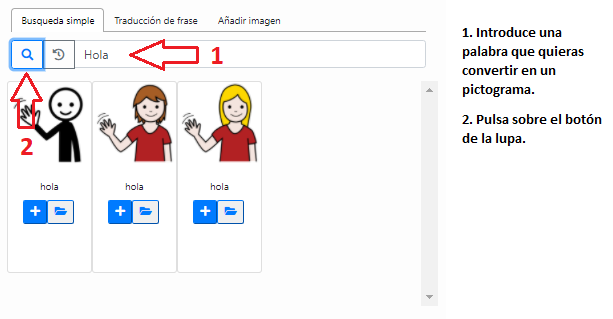
\includegraphics[width=0.8\linewidth]{Imagenes/Bitmap/evaluacionPista}
	\caption{ Ejemplo de pista en el formulario: Buscar un pictograma.
	}
	\label{fig:evaPista}
\end{figure} 

Cada una de las tareas del formulario cuenta con una serie de pistas que indican como completar una acción mediante una URL asociada a una imagen. De esta manera el usuario puede resolver una duda concreta y no se desvela cómo completar otras acciones dentro de la tarea. Otra manera de orientar al usuario para darle a conocer si ha realizado la tarea correctamente, fue mediante imágenes que mostraran un posible estado final del tablero o componente al completar la tarea.


Respecto a las tareas, aunque no se abarcan todas las posibilidades que ofrece la herramienta, sí representa una muestra significativa de las funcionalidades disponibles en la aplicación. Esto se debe a que el formulario debe de completarse en un período razonable de tiempo y no extenderse más de lo debido. 
A continuación se detallarán las tareas escogidas y el motivo de elección: 

\begin{itemize}
	\item \textbf{Tarea 1, Buscar un pictograma, añadirlo al tablero y editarlo}: se trata de la funcionalidad más básica de la aplicación.
	\item \textbf{Tarea 2, Crear una lista de pictos, añadir un pictograma a una lista de pictos y añadir un pictograma de la lista al tablero}: una funcionalidad que ha causado dudas durante el desarrollo, ya que se desconocía si era lo suficientemente claro su funcionamiento.
	\item \textbf{Tarea 3, Traducir una frase, añadirla al tablero y ocultar un pictograma de la frase}: al ser una funcionalidad más compleja y con más opciones era deseable conocer el desempeño del usuario con ella.
	\item \textbf{Tarea 4, Añadir fotos, figuras e iconos al tablero}: abarcan funciones independientes más simples comparadas con las anteriores, ya que requieren menos acciones para completarlas.
\end{itemize}
El tipo de cuestionario seleccionado para medir la usabilidad de cada tarea ha sido el ASQ\footnote{\url{https://help.qualaroo.com/hc/en-us/articles/360039070552-After-Scenario-Questionnaire-ASQ-}} (After Scenario Questionnaire), el cual permite al usuario evaluar la dificultad de cada una de ellas. Este cuestionario ha de ser respondido una vez finalizada cada tarea y está compuesto por tres afirmaciones. El usuario ha de indicar cuán de acuerdo está mediante una escala de 1 a 7, siendo el 1 muy en desacuerdo y el 7 muy de acuerdo. Dichas afirmaciones son: 

\begin{enumerate}
	\item En general, estoy satisfecho con la facilidad para completar la tarea en este escenario.
	\item En general, estoy satisfecho con la cantidad de tiempo que tomó completar la tarea en este escenario.
	\item Estoy satisfecho con la respuesta de la web al realizar una acción, sé lo que pasa en todo momento.
\end{enumerate}

Esta última afirmación fue modificada para ser ajustada al contexto de la aplicación, enfocándose más al feedback que pueda aportar la tarea. Originalmente ésta era:  \textit{En general, estoy satisfecho con la información de soporte (ayuda en línea, mensajes y documentación) al completar la tarea}

Tras completar las tareas, se ofrece al usuario a que siga probando la aplicación con libertad para probar el resto de funcionalidades que no aparecieran en las tareas.  
También se realizan algunas preguntas de respuesta libre por si se ha sentido perdido o ha echado en falta alguna función durante la realización de las tareas.  

Por último, de manera opcional, se propone al usuario otro formulario donde puede dar su opinión sobre la aplicación de manera global. Para ello se ha utilizado las preguntas del cuestionario de usabilidad  SUS\footnote{\url{https://help.qualaroo.com/hc/en-us/articles/360039474571-System-Usability-Scale-SUS-}} (System Usability Scale), que mide la usabilidad del sistema. Nuevamente se plantea una serie de afirmaciones, en este caso 10, donde el usuario deberá elegir en una escala de 1 a 5 cuán de acuerdo está con ellas. Dichas afirmaciones son: 


\begin{enumerate}
		\item Creo que usaría esta web frecuentemente.
	\item Encontré la web innecesariamente compleja.
	\item Creo que la web es fácil de usar.
	\item Creo que necesitaría la ayuda de una persona con conocimientos técnicos para usar la web.
	\item Las funciones de la web están bien integradas.
	\item Creo que la web es muy confusa.
	\item Creo que la mayoría de la gente aprendería a usar la web muy rápidamente.
	\item Encuentro la web muy complicada de utilizar.
	\item Me siento confiado/a al utilizar la web.
	\item Necesito aprender muchas cosas antes de poder utilizar la web.
\end{enumerate}

Una vez acabado el cuestionario, éste fue enviado. Tras dos semanas, se obtuvieron más de 36 respuestas por parte de estudiantes y profesores. 

\textcolor{red}{Introducción a los 2 grupos}


\section{Resultados de la evaluación}
\label{eva:res}

El día 1 de junio se cerró el formulario, y en el repositorio de GitHub del proyecto\footnote{\url{https://github.com/NILGroup/TFG-2021-EditorPictogramas/blob/master/Respuestas\%20de\%20la\%20Evaluaci\%C3\%B3n\%20PictUp!.xlsx}} se puede encontrar el archivo con todas las respuestas obtenidas. A continuación se expondrán los resultados obtenidos. Como se ha explicado anteriormente, los usuarios que contestaron fueron divididos en dos grupos. Un primer grupo compuesto por seis personas que crean y usan material criptográfico y un segundo grupo de 33 usuarios que no crea ni utiliza material. 

\subsection{Resultados del cuestionario ASQ}
Las Tablas \ref{tab:area1respuestas} a \ref{tab:area4respuestas} representan los resultados de cada tarea, teniendo en cuenta que la nota ASQ de cada tarea es calculada mediante la media de las tres preguntas. En cada una puede verse los resultados de los dos grupos respecto a la puntuación media y varianza del cuestionario ASQ. También se incluye el porcentaje de utilización de las pistas en cada grupo, que servirá para concretar que acciones de cada tarea resultaron más confusas.


\begin{table}

\begin{tabular}{ |p{4cm}|p{2cm}|p{2cm}|p{2cm}|p{2cm}|  }
	\hline
	\multicolumn{5}{|c|}{Tarea 1: Búsqueda y edición de pictograma} \\
	\hline
	 & \multicolumn{2}{p{4cm}|}{Grupo de usuarios que crean y usan material pictográfico} & \multicolumn{2}{p{4cm}|}{Grupo del resto de usuarios }  \\ 
	\hline
	 Preguntas ASQ & Puntuación media  &Desviación típica de la puntuación & Puntuación media & Desviación típica de la puntuación\\
	\hline
	1. En general, estoy satisfecho con la facilidad de completar esta tarea &6.5  &0.836 &6.111  &1.012\\
	\hline
	2. En general estoy satisfecho con la cantidad de tiempo que me ha llevado completar esta tarea&6.5  &0.836  &6.333 &0.919\\
	\hline
	3. Estoy satisfecho con la respuesta de la web al realizar una acción, sé lo que pasa en todo momento &6.5 &0.836 & 6.259  &1.095\\
	\hline
	Nota final &6.5 &0.836 &6.234  &0.890\\
	\hline
	\multicolumn{5}{|c|}{Uso de pistas en Tarea 1} \\
	\hline
	& \multicolumn{2}{p{4cm}|}{Grupo de usuarios que crean y usan material pictográfico} & \multicolumn{2}{p{4cm}|}{Grupo del resto de usuarios }  \\ 
	\hline
	 Pistas &Nº de usos de la pista &\% de uso de la pista&Nº de usos de la pista&\% de uso de la pista\\
	\hline
	Pista 1: Buscar pictograma &2  &33.33\% &5  &18.51\%\\
	\hline
	Pista 2: Añadir al tablero &4  &66.66\%  &2 &7.40\%\\
	\hline
	Pista 3: Editar picto &1 &16.66\% &4  &14.81\%\\
	\hline
\end{tabular}
\caption{\label{tab:area1respuestas}Tabla de los resultados de la Tarea 1}
\end{table}

\begin{table}
\begin{tabular}{ |p{4cm}|p{2cm}|p{2cm}|p{2cm}|p{2cm}|  }
	\hline
	\multicolumn{5}{|c|}{Tarea 2: Listas de pictogramas} \\
	\hline
	& \multicolumn{2}{p{4cm}|}{Grupo de usuarios que crean y usan material pictográfico} & \multicolumn{2}{p{4cm}|}{Grupo del resto de usuarios }  \\ 
	\hline
	Preguntas ASQ & Puntuación media  &Desviación típica de la puntuación & Puntuación media & Desviación típica de la puntuación\\
	\hline
	1. En general, estoy satisfecho con la facilidad de completar esta tarea &6.333  &0.816 &5.592 &1.393\\
	\hline
	2. En general estoy satisfecho con la cantidad de tiempo que me ha llevado completar esta tarea &6.666  &0.516 &5.703 &1.353\\
	\hline
	3. Estoy satisfecho con la respuesta de la web al realizar una acción, sé lo que pasa en todo momento &6.333 &0.816 &5.629   &1.305\\
	\hline
	Nota final &6.444 &0.688 &5.641  &1.194\\
	\hline
	\multicolumn{5}{|c|}{Uso de pistas en Tarea 2} \\
	\hline
	& \multicolumn{2}{p{4cm}|}{Grupo de usuarios que crean y usan material pictográfico} & \multicolumn{2}{p{4cm}|}{Grupo del resto de usuarios }  \\ 
	\hline
	Pistas &Nº de usos de la pista &\% de uso de la pista&Nº de usos de la pista&\% de uso de la pista\\
	\hline
	Pista 1: ¿Dónde crear una lista de pictogramas? &5  &83.33\% &12 &44.44\%\\
	\hline
	Pista 2: ¿Cómo crear y cómo añadir un pictograma a una lista? &3  &50\%  &7 &25.92\%\\
	\hline
	Pista 3: ¿Dónde añadir un picto desde la lista? &4 &66.66\% &4  &14.81\%\\
	\hline
\end{tabular}
\caption{\label{tab:area2respuestas}Tabla de los resultados de la Tarea 2}
\end{table}


\begin{table}
\begin{tabular}{ |p{4cm}|p{2cm}|p{2cm}|p{2cm}|p{2cm}|  }
	\hline
	\multicolumn{5}{|c|}{Tarea 3: Traducir frase a pictogramas} \\
	\hline
	& \multicolumn{2}{p{4cm}|}{Grupo de usuarios que crean y usan material pictográfico} & \multicolumn{2}{p{4cm}|}{Grupo del resto de usuarios }  \\ 
	\hline
	Preguntas ASQ & Puntuación media  &Desviación típica de la puntuación & Puntuación media & Desviación típica de la puntuación\\
	\hline
	1. En general, estoy satisfecho con la facilidad de completar esta tarea &5.833  &2.401 &5.851  &1.350\\
	\hline
	2. En general estoy satisfecho con la cantidad de tiempo que me ha llevado completar esta tarea &6.833  &0.408 &6.148 &1.199\\
	\hline
	3. Estoy satisfecho con la respuesta de la web al realizar una acción, sé lo que pasa en todo momento &5.333 &2.658 &5.925  &1.141\\
	\hline
	Nota final &6 &1.673 &5.975 &1.025\\
	\hline
	\multicolumn{5}{|c|}{Uso de pistas en Tarea 3} \\
	\hline
	& \multicolumn{2}{p{4cm}|}{Grupo de usuarios que crean y usan material pictográfico} & \multicolumn{2}{p{4cm}|}{Grupo del resto de usuarios }  \\ 
	\hline
	Pistas &Nº de usos de la pista &\% de uso de la pista&Nº de usos de la pista&\% de uso de la pista\\
	\hline
	Pista 1: ¿Cómo traducir una frase a picto? &1  &16.66\% &4  &14.81\%\\
	\hline
	Pista 2: ¿Cómo cambiar un picto de la frase por otro alternativo? &1  &16.66\%  &3 &11.11\%\\
	\hline
	Pista 3: ¿Cómo añadir la frase al tablero? &1 &16.66\% &6   &22.22\%\\
	\hline
	Pista 4: ¿Cómo ocultar un picto de la frase? &3 &50\% &5   &18.51\%\\
	\hline

\end{tabular}
\caption{\label{tab:area3respuestas}Tabla de los resultados de la Tarea 3}
\end{table}

\begin{table}

\begin{tabular}{ |p{4cm}|p{2cm}|p{2cm}|p{2cm}|p{2cm}|  }
	\hline
	\multicolumn{5}{|c|}{Tarea 4: Fotos, figuras e iconos} \\
	\hline
	& \multicolumn{2}{p{4cm}|}{Grupo de usuarios que crean y usan material pictográfico} & \multicolumn{2}{p{4cm}|}{Grupo del resto de usuarios }  \\ 
	\hline
	Preguntas ASQ & Puntuación media  &Desviación típica de la puntuación & Puntuación media & Desviación típica de la puntuación\\
	\hline
	1. En general, estoy satisfecho con la facilidad de completar esta tarea &6.166  &0.752 &6.444  &0.800\\
	\hline
	2. En general estoy satisfecho con la cantidad de tiempo que me ha llevado completar esta tarea &6.333  &0.816  &6.444 &0.847\\
	\hline
	3. Estoy satisfecho con la respuesta de la web al realizar una acción, sé lo que pasa en todo momento &6 &1.549 &6.518   &0.935\\
	\hline
	Nota final &6.166 &1.005 &6.469  &0.758\\
	\hline
	\multicolumn{5}{|c|}{Uso de pistas en Tarea 4} \\
	\hline
	& \multicolumn{2}{p{4cm}|}{Grupo de usuarios que crean y usan material pictográfico} & \multicolumn{2}{p{4cm}|}{Grupo del resto de usuarios }  \\ 
	\hline
	Pistas &Nº de usos de la pista &\% de uso de la pista&Nº de usos de la pista&\% de uso de la pista\\
	\hline
	Pista 1: ¿Cómo añadir una imagen con su texto? &2  &33.33\% &2 &7.40\%\\
	\hline
	Pista 2: ¿Cómo añadir un texto al tablero y seleccionar la fuente? &1 &16.66\%  &4 &14.81\%\\
	\hline
	Pista 3: ¿Cómo añadir una figura? &3 &50\% &3   &11.11\% \\
	\hline
\end{tabular}
\caption{\label{tab:area4respuestas}Tabla de los resultados de la Tarea 4}
\end{table}

\subsection{Resultados del cuestionario SUS}
Al igual que en ASQ,  la Tabla \ref{tab:cuestionarioSUS} se mostrarán los resultados de ambos grupos en cada pregunta. Para obtener el resultado total del cuestionario SUS se debe de calcular en función del tipo de pregunta, es decir, las preguntas pares se calcularán restando cinco menos el valor dado por los usuarios y las preguntas impares se le restará uno al valor dado por los usuarios.  Esta distinción a la hora de calcular el resultado es debido a que las preguntas se intercalan con connotaciones positivas y negativas para obligar al usuario a pensar detenidamente las respuestas\footnote{\url{https://measuringu.com/10-things-sus/}}.



\begin{table}
	
	\begin{tabular}{ |p{4cm}|p{2cm}|p{2cm}|p{2cm}|p{2cm}|  }
		\hline
		\multicolumn{5}{|c|}{Resultados del cuestionario SUS} \\
		\hline
		& \multicolumn{2}{p{4cm}|}{Grupo de usuarios que crean y usan material pictográfico} & \multicolumn{2}{p{4cm}|}{Grupo del resto de usuarios }  \\ 
		\hline
		Preguntas & Puntuación media  &Desviación típica de la puntuación & Puntuación media & Desviación típica de la puntuación\\
		\hline
		1. Creo que usaría esta web frecuentemente &4.166 &0.752 &3  &1.296\\
		\hline
		2. Encontré la web innecesariamente compleja &1.166  &0.408  &1.592 &1.047\\
		\hline
		3. Creo que la web es fácil de usar &4.5 &0.836 &4.518  &0.509\\
		\hline
		4. Creo que necesitaría la ayuda de una persona con conocimientos técnicos para usar la web &1.166 &0.408 &1.629  &1.079\\
		\hline
		5. Las funciones de la web están bien integradas &3.6 &0.894 &4.592 &0.572\\
		\hline
		6. Creo que la web es muy confusa &1.333  &0.816 &1.444 &0.640\\
		\hline
		7. Creo que la mayoría de la gente aprendería a usar la web muy rápidamente &4.666 &0.516  &4.518 &0.752\\
		\hline
		8. Encuentro la web muy complicada de utilizar &1 &0 &1.555 &1.0127 \\
		\hline
		9. Me siento confiado/a al utilizar la web &4 &1.549 &4.444  &0.800 \\
		\hline
		10. Necesito aprender muchas cosas antes de poder utilizar la web &1.166 &0.408 &1.555  &0.933 \\
		\hline
		Puntuación final &86.25 &11.48368408 &82.962 &12.596 \\
		\hline
	\end{tabular}
\caption{\label{tab:cuestionarioSUS}Tabla de los resultados del cuestionario SUS.}	
\end{table}


\subsection{Observaciones de los usuarios}
\label{cap6:sec:observaciones}
Respecto a los campos de respuesta abierta donde que permitían a los usuarios indicar en qué momento se han sentido perdidos o desorientados  y qué elementos echaban en falta, cementamos a continuación las respuestas más frecuentes. 

Por parte de los usuarios que crean material pictográfico, la mayoría no se sintió perdido durante la realización de las tareas. Aunque se apuntó que confundía el hecho que al añadir varios pictogramas al tablero se superpusieran. 

Respecto a funcionalidades que echaban en falta se mencionaron: 
\begin{itemize}
	\item Ajustar el tamaño de la letra en las frases e imágenes. 
	\item La posibilidad en las frases de pictogramas de asignar la palabra de un pictograma a su pictograma correspondiente. 
	\item Permitir agrupar elementos del tablero para ser desplazados con comodidad.
	\item Eliminar todos los elementos del tablero mediante un botón, en vez de eliminarlos uno a uno.
	\item Leyenda de significados de los colores, pues cada color está asignado a verbos, sustantivos, adjetivos, etc. De esta manera el usuario no tendría que memorizar el significado de cada color.
\end{itemize}


El grupo mayoritario compuesto por los usuarios que no crean o usan material pictográfico ofrece una información muy útil para saber si la aplicación es fácil de utilizar. Respecto a sus respuestas sobre cuándo se sentían más perdidos, principalmente se daba por tres motivos. La primera se daba únicamente al principio, tras un breve período de uso la aplicación se utilizaba con facilidad. El segundo motivo que más confusión ha generado ha sido al crear y añadir pictogramas a las listas de pictogramas. La tercera funcionalidad que más problemas ha causado ha sido al colocar una frase de pictogramas al tablero y la edición de esta. 

Respecto a las funcionalidades que ha echado en falta este segundo grupo de usuarios:

\begin{itemize}
	\item Posibilidad de buscar y añadir imágenes de Internet dentro de la web.
	\item Posibilidad de arrastrar los elementos desde la barra de herramientas al tablero.
	\item Al pulsar intro no se realiza la búsqueda. Este tipo de atajos de teclado son de utilidad.
	\item Edición del texto de las fotos y su tipo de letra.
	\item Cambiar el color de fondo del tablero.
	\item Posibilidad de quitar un pictograma de la frase antes de añadirla al tablero.
	\item Posibilidad de cambiar el tamaño del tablero.
	\item Botón para eliminar todos los elementos del tablero.
	\item La traducción no es del todo precisa.
	\item Posibilidad de añadir rectángulos.
	\item Posibilidad de añadir un pictograma a una lista de pictogramas desde la traducción de frase. 
\end{itemize}

\section{Evaluación adicional}
\label{cap6:sec:evaluacion}
\textcolor{red}{Evaluación libre}


Aparte de los resultados obtenidos por la encuesta, también contamos con observaciones y comentarios por parte de un grupo de ocho profesores de educación especial. Éstos probaron la aplicación sin realizar el formulario, por lo que su uso fue totalmente libre. Transmitieron que les gustaba la aplicación, aunque había algunos aspectos que echaban en falta y que se detallan a continuación: 

\begin{itemize}
	\item Posibilidad de quitar las líneas de la cuadrícula, pues cuando se descarga e imprime el tablero éstas pueden distraer o confundir al usuario.  
	\item Un nuevo componente que permita asociar un pictograma con una imagen en movimiento o vídeo.
		\item Buscador integrado de imágenes, para buscar y añadir imágenes igual de rápido que con los pictogramas. De esta manera se evitaría descargar una imagen y subirla a PictUp! como foto. 
	\item El funcionamiento de la cuadrícula es correcto, pero se prefiere un modo de edición más similar al de Power Point o Canvas. Donde se colocan todos los elementos de manera proporcional y se alinean automáticamente.
	\item Posibilidad de poder poner cualquier color a los bordes, la selección actual a seis colores limita su uso.
	\item Posibilidad de cambiar el color de fondo de un pictograma con cualquier color. 
	\item Permitir la reproducción de frases en el elemento que representa una frase de pictogramas. La reproducción de la frase puede ser hecha mediante un sintetizador de texto a voz. Esto permitiría a los usuarios asociar el sonido de una palabra a la imagen.
	\item Posibilidad de poder cambiar el tamaño del tablero, ya que puede quedarse pequeño si se añaden muchos elementos.
	\item Añadir tipografías fáciles de leer, como OpenDyslexic que facilita la lectura a personas disléxicas. Se menciona que las letras espaciadas son fáciles de leer. 
	\item Crear un tutorial para YouTube donde se explique detalladamente las funcionalidades de PictUp!. 
	\item Les gustaría que hubiera iconos de caras, como cara riendo, llorando o contenta. 
\end{itemize}






\section{Análisis de los resultados}
\label{eva:analisis}


Tras recopilar la información, se analizó la usabilidad y facilidad de uso de la aplicación en base a las métricas obtenidas y los comentarios. También se identificaron las funcionalidades más conflictivas para ser mejoradas en un futuro. 

Para conocer la usabilidad general de la aplicación, se utilizaron las notas finales obtenidas en el cuestionario SUS. En ambos grupos se ha obtenido resultados similares: el grupo que crea y utiliza material pictográfico ha puntuado la usabilidad con 86,25 puntos de media y el segundo grupo que no los crea ni utiliza con una puntuación de 82,9. Según el estándar\footnote{\url{https://www.usabilitest.com/system-usability-scale}} de SUS, las puntuaciones superiores a 80,2 corresponden a una usabilidad excelente. 


Mediante la nota ASQ se puede saber la facilidad de uso de cada tarea. A continuación, se analizarán los resultados de cada tarea de manera individual.

\begin{itemize}
	\item La primera tarea contó con respuestas positivas en ambos grupos, con un resultado ASQ superior a 6 de media. Respecto al uso de las pistas, no se usaron muchas, aunque en el grupo de usuarios que crea y usa material tuvieron complicaciones al encontrar el botón de añadir un pictograma al tablero. Esto puede atribuirse a ser la primera vez que se realiza la acción de añadir elementos al tablero, ya que en las siguientes tareas este problema no vuelve a ocurrir. 
	
	\item La segunda tarea contó con una menor puntuación ASQ por parte de los usuarios que no utilizan material pictográfico. El uso de las pistas demuestra que la principal dificultad planteada en esta tarea se debe a la creación de listas de pictogramas, siendo la más utilizada por ambos grupos. Esto se debe a que el botón de carpeta dentro del pictograma no ha sido tan intuitivo como se esperaba.
	
	
	\item La tercera tarea de traducción de frase a pictograma ha sido bien valorada de manera general, pero la respuesta de la web al realizar una acción tuvo una puntuación inferior respecto al resto de preguntas. En base al uso de las pistas, esto es debido a que al colocar la frase al tablero no ha sido fácil de añadir al tablero, al igual que el botón para ocultar un pictograma de la frase.
	
	
	\item La cuarta tarea tuvo respuestas muy positivas. El porcentaje de usuarios que utilizaron pistas para resolver las tareas fue muy bajo. En base a los resultados del cuestionario ASQ podemos concluir que la usabilidad correspondiente a esta tarea es muy alta.
\end{itemize}

Los problemas de usabilidad detectados fueron contrastados mediante los comentarios ofrecidos por ambos grupos. Finalmente se puede concluir que excluyendo algunas dificultades, en general la aplicación es lo suficientemente fácil de utilizar.
